\documentclass[a4paper,12pt]{article}
\usepackage{graphicx} % Required for inserting images
\usepackage{geometry} % Required for setting margins
\usepackage{pdflscape} % Required to change certain pages into landscape/portrait mode

\geometry{
	a4paper,
	total={170mm,242mm},
	left=20mm,right=20mm,
	top=20mm,bottom=25mm
}

\begin{document}
\begin{center}
\large{\textbf{Product Backlog and Sprint Plan}}
\end{center}
\normalsize 
A product backlog is a list of features or tasks that need to be done to deliver a valuable product to the customer. It is prioritized by the product owner based on the business value, user needs, and technical feasibility of each feature.

Here is a possible product backlog for your system, using the MoSCoW method to prioritize the features:
\begin{table}[!h]
\centering
\begin{tabular}{|l|p{10cm}|l|}
\hline
\textbf{Feature} & \textbf{Description} & \textbf{Priority} \\
\hline
User registration & Provide a way to register user data, such as name, email, password, role (consumer or producer), and preferences. & Must have \\
\hline
User authentication & Provide a way to verify the identity of the user and grant access to the system. & Must have \\
\hline
User profile & Provide a way to view and edit the user data and preferences. & Must have \\
\hline
Service declaration & Provide a way for a producer to declare offered services, such as name, description, duration, price, and availability. & Must have \\
\hline
Service browsing & Provide a way for a consumer to look for available services, using filters, categories, and keywords. & Must have \\
\hline
Event creation & Provide a way for a producer to create new events, either public or private, based on the offered services and the availability. & Must have \\
\hline
Event booking & Provide a way for a consumer to book an event, either public or private, based on the available services and the time slots. & Must have \\
\hline
Event cancellation & Provide a way for a producer or a consumer to cancel an event or a booking, with a notification to the other party. & Must have \\
\hline
Event payment & Provide a way for a consumer to pay for an attended event, using a secure payment method. & Must have \\
\hline
Event notification & Provide a way to send consumers notifications about booked events, such as reminders, confirmations, or cancellations. & Should have \\
\hline
Event message & Provide a way for a producer to create notifications about an event, such as broadcast messages, updates, or feedback requests. & Should have \\
\hline
Event survey & Provide a way to collect surveys about completed events, such as ratings, reviews, or suggestions. & Should have \\
\hline
Data analytics & Provide a way to provide data analytics obtained by the system to producers, such as number of bookings, revenue, customer satisfaction, or trends. & Could have \\
\hline
Web interface & Provide a web application interface to use the system, using a responsive and user-friendly design. & Must have \\
\hline
Mobile interface & Provide a mobile application interface to use the system, using a native or hybrid approach. & Could have \\
\hline
\end{tabular}
\end{table}

\newpage\noindent
Here is a possible sprint plan for your system, using the Scrum framework and assuming a team of 5 people and a sprint length of 4 weeks:
\begin{table}[!h]
\centering
\begin{tabular}{|c|p{5cm}|p{7cm}|p{2cm}|}
\hline
\textbf{Sprint} & \textbf{Goal} & \textbf{Features}& \textbf{Estimated effort} \\
\hline
1 & To enable users to register, authenticate, and manage their profiles. & User registration, User authentication, User profile, Web interface (for these features) & 80 hours \\
\hline
2 & To enable producers to declare and create events, and consumers to browse and book events. & Service declaration, Service browsing, Event creation, Event booking, Web interface (for these features) & 120 hours \\
\hline
3 & To enable users to cancel, pay, and receive notifications for events. & Event cancellation, Event payment, Event notification, Event message, Web interface (for these features) & 100 hours \\
\hline
\end{tabular}
\end{table}\\
More in detail, here is a possible example of the product backlog divided into 3 sprints:
\begin{itemize}
	\vspace{-0.3cm}
	\item Sprint 1: The goals of this sprint is to enable users to register, authenticate, and manage their profiles. The product backlog items for this sprint are:
		\begin{itemize}
			\vspace{-0.3cm}
			\item As a user, I want to register into the system using name, email, password, role (consumer or producer), and preferences, so that I can access the system easily and securely.
			\vspace{-0.2cm}
			\item As a user, I want to authenticate into the system, so that I have access to the system.
			\vspace{-0.6cm}
			\item As a user, I want to view and edit the user data and preferences, so that I can update my personal information.
			\vspace{-0.2cm}
			\item As a user, I want to see a modern and responsive web design, so that I can use the system on any device and browser.
		\end{itemize}
	\vspace{-0.3cm}
	\item Sprint 2: The goals of this sprint is to enable producers to declare and create events, and consumers to browse and book events. The product backlog items for this sprint are:
		\begin{itemize}
			\vspace{-0.3cm}
			\item As a producer, I want to declare offered services, so that I satisfy customers by providing them with valuable solutions that meet their needs and preferences.
			\vspace{-0.2cm}
			\item As a consumer, I want to look for available services, using filters, categories, and keywords, so that I can find and book the best solution that meets my needs and preferences.
			\vspace{-0.2cm}
			\item As a producer, I want to create new events, either public or private, based on the offered services and the availability, so that I can generate more revenue and customer loyalty by offering diverse and customized solutions that cater to different needs and preferences.
			\item As a consumer, I want to book an event, either public or private, based on the available services and the time slots, so that I can secure my spot and enjoy the benefits of the service I'm interested in.
		\end{itemize}
	\vspace{-0.3cm}
	\item Sprint 3: The goals of this sprint is to enable users to cancel, pay, and receive notifications for users. The product backlog items for this sprint are:
		\begin{itemize}
			\vspace{-0.3cm}
			\item As a producer or a consumer, I want to cancel an event or a booking, with a notification to the other party, so that I can reschedule or reorganize the event or booking, due to changes in availability, demand, or preferences.
			\vspace{-0.2cm}
			\item As a consumer, I want to pay for an attended event, using a secure payment method, so that I can pay easily and securely.
			\vspace{-0.2cm}
			\item As a producer, I want to send consumers notifications about booked events, such as reminders, confirmation, or cancellations, so that I can enhance customer satisfaction by providing timely and relevant information that helps them prepare for and enjoy the event.
			\item As a producer, I want to create notifications about an event, such as broadcast messages, updates, or feedback requests, so that I can increase customer engagement by providing them with valuable and relevant information that enhances their event experience.
		\end{itemize}
\end{itemize}
The specific product backlog items that the Scrum team will work on in the next sprint are agreed to at spring planning, which ocurs at the beginning of each sprint. During this activity, the team generates a spring backlog: a description of the task-level work that has to be completed to get the product backlog items done (see Figure \ref{fig:01}).
\begin{figure}[!h]
\centering
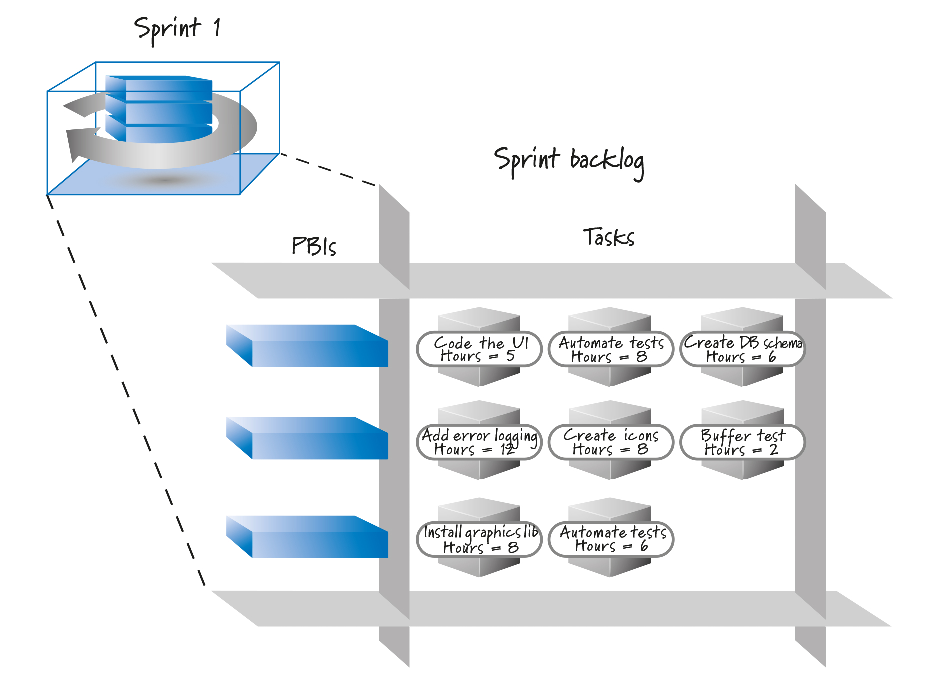
\includegraphics[scale=0.8]{Sprint Backlog.pdf}
\caption{Each sprint has a sprint backlog}
\label{fig:01}
\end{figure}\\
A sprint backlog is a list of tasks that the team commits to complete in a sprint. Each task is derived from a feature or user story in the sprint plan, and has a clear definition of done, an owner, and an estimated effort. The team updates the sprint backlog daily to track the progress and status of each task.

Here is a possible sprint backlog for each sprint, based on the features and estimated effort in the sprint plan:

\newpage\noindent
\begin{landscape}
\begin{table}[!h]
\centering
\begin{tabular}{|c|l|p{7cm}|p{6cm}|l|p{2cm}|}
\hline
\textbf{Sprint} & \textbf{Feature} & \textbf{Task} & \textbf{Definition of done} & \textbf{Owner} & \textbf{Estimated effort} \\
\hline
1 & User registration & Design the user registration form & The form has fields for name, email, password, role, and preferences, and validates the input & UI designer & 8 hours \\
\hline
1 & User registration & Implement the user registration logic & The logic checks the input, encrypts the password, and stores the user data in the database & Programmer & 16 hours \\
\hline
1 & User registration & Test the user registration functionality & The functionality works as expected, with no errors or bugs & Tester & 8 hours \\
\hline
1 & User authentication & Design the user login page & The page has fields for email and password, and a button to login & UI designer & 4 hours \\
\hline
1 & User authentication & Implement the user authentication logic & The logic verifies the email and password, and grants access to the system & Programmer & 8 hours \\
\hline
1 & User authentication & Test the user authentication functionality & The functionality works as expected, with no errors or bugs & Tester & 4 hours \\
\hline
1 & User profile & Design the user profile page & The page shows the user data and preferences, and has buttons to edit or delete them & UI designer & 8 hours \\
\hline
1 & User profile & Implement the user profile logic & The logic retrieves, updates, or deletes the user data and preferences from the database & Programmer & 16 hours \\
\hline
1 & User profile & Test the user profile functionality & The functionality works as expected, with no errors or bugs & Tester & 8 hours \\
\hline
1 & Web interface & Integrate the user registration, authentication, and profile pages & The pages are linked and consistent with the web design standards & UI designer & 8 hours \\
\hline
2 & Service declaration & Design the service declaration form & The form has fields for name, description, duration, price, and availability, and validates the input & UI designer & 8 hours \\
\hline
\end{tabular}
\end{table}
\end{landscape}

\newpage\noindent
\begin{landscape}
\begin{table}[!h]
\centering
\begin{tabular}{|c|l|p{7cm}|p{6cm}|l|p{2cm}|}
\hline
\textbf{Sprint} & \textbf{Feature} & \textbf{Task} & \textbf{Definition of done} & \textbf{Owner} & \textbf{Estimated effort} \\
\hline
2 & Service declaration & Implement the service declaration logic & The logic checks the input and stores the service data in the database & Programmer & 16 hours \\
\hline
2 & Service declaration & Test the service declaration functionality & The functionality works as expected, with no errors or bugs & Tester & 8 hours \\
\hline
2 & Service browsing & Design the service browsing page & The page shows the available services, with filters, categories, and keywords & UI designer & 8 hours \\
\hline
2 & Service browsing & Implement the service browsing logic & The logic retrieves the service data from the database and applies the filters, categories, and keywords & Programmer & 16 hours \\
\hline
2 & Service browsing & Test the service browsing functionality & The functionality works as expected, with no errors or bugs & Tester & 8 hours \\
\hline
2 & Event creation & Design the event creation form & The form has fields for service, date, time, type, and capacity, and validates the input & UI designer & 8 hours \\
\hline
2 & Event creation & Implement the event creation logic & The logic checks the input and stores the event data in the database & Programmer & 16 hours \\
\hline
2 & Event creation & Test the event creation functionality & The functionality works as expected, with no errors or bugs & Tester & 8 hours \\
\hline
2 & Event booking & Design the event booking page & The page shows the details of the event, and has a button to book it & UI designer & 4 hours \\
\hline
2 & Event booking & Implement the event booking logic & The logic verifies the availability and stores the booking data in the database & Programmer & 8 hours \\
\hline
2 & Event booking & Test the event booking functionality & The functionality works as expected, with no errors or bugs & Tester & 4 hours \\
\hline
\end{tabular}
\end{table}
\end{landscape}

\newpage\noindent
\begin{landscape}
\begin{table}[!h]
\centering
\begin{tabular}{|c|l|p{7cm}|p{6cm}|l|p{2cm}|}
\hline
\textbf{Sprint} & \textbf{Feature} & \textbf{Task} & \textbf{Definition of done} & \textbf{Owner} & \textbf{Estimated effort} \\
\hline
2 & Web interface & Integrate the service declaration, browsing, creation, and booking pages & The pages are linked and consistent with the web design standards & UI designer & 8 hours \\
\hline
3 & Event cancellation & Design the event cancellation page & The page shows the details of the event, and has a button to cancel it & UI designer & 4 hours \\
\hline
3 & Event cancellation & Implement the event cancellation logic & The logic deletes the event or booking data from the database, and sends a notification to the other party & Programmer & 8 hours \\
\hline
3 & Event cancellation & Test the event cancellation functionality & The functionality works as expected, with no errors or bugs & Tester & 4 hours \\
\hline
3 & Event payment & Design the event payment page & The page shows the details of the event, and has a button to pay for it & UI designer & 4 hours \\
\hline
3 & Event payment & Implement the event payment logic & The logic verifies the attendance and processes the payment using a secure method & Programmer & 8 hours \\
\hline
3 & Event payment & Test the event payment functionality & The functionality works as expected, with no errors or bugs & Tester & 4 hours \\
\hline
3 & Event notification & Design the event notification page & The page shows the notifications about booked events, such as reminders, confirmations, or cancellations & UI designer & 4 hours \\
\hline
3 & Event notification & Implement the event notification logic & The logic sends and receives notifications about booked events, using email or SMS & Programmer & 8 hours \\
\hline
3 & Event notification & Test the event notification functionality & The functionality works as expected, with no errors or bugs & Tester & 4 hours \\
\hline
\end{tabular}
\end{table}
\end{landscape}

\newpage\noindent
\begin{landscape}
\begin{table}[!h]
\centering
\begin{tabular}{|c|l|p{7cm}|p{6cm}|l|p{2cm}|}
\hline
\textbf{Sprint} & \textbf{Feature} & \textbf{Task} & \textbf{Definition of done} & \textbf{Owner} & \textbf{Estimated effort} \\
\hline
3 & Event message & Design the event message page & The page shows the messages about an event, such as broadcast messages, updates, or feedback requests & UI designer & 4 hours \\
\hline
3 & Event message & Implement the event message logic & The logic sends and receives messages about an event, using email or SMS & Programmer & 8 hours \\
\hline
3 & Event message & Test the event message functionality & The functionality works as expected, with no errors or bugs & Tester & 4 hours \\
\hline
3 & Web interface & Integrate the event cancellation, payment, notification, and message pages & The pages are linked and consistent with the web design standards & UI designer & 8 hours \\
\hline
\end{tabular}
\end{table}
\end{landscape}





\end{document}
